\chapter{Cronograma}\label{cronograma}

O início do desenvolvimento foi definido para o início de Março de 2024, a partir de uma reunião externa com funcionários do Ceclimar, para definição do escopo geral do projeto.

A partir do dia 5 de Maio ficou definido o início do desenvolvimento do trabalho com a revisão bibliográfica (prazo máximo Julho), definição metodológica, o levantamento de requisitos (prazo máximo Agosto) e a organização da implementação (prazo máximo Junho). O levantamento de requisitos do sistema terá um prazo mais prolongado para que os alinhamentos de definições com a equipe do Ceclimar sejam mais abertos e constantes.

O desenvolvimento do sistema terá seu início no dia 1º de Maio e sua projeção final programada para a última metade de Outubro. Aliado a isto, será iniciada a redação do trabalho a partir dos dados coletados na revisão bibliográfica, levantamento de requisitos e regras de negócio e definição metodológica. A parte escrita tem o prazo limite de finalização marcado para o final de novembro, mês em que também se iniciará a revisão do mesmo. A projeção é de que o projeto esteja pronto em dezembro para que a apresentação final seja agendada para o final do segundo semestre letivo.

\begin{figure}[htb]
  \centering
  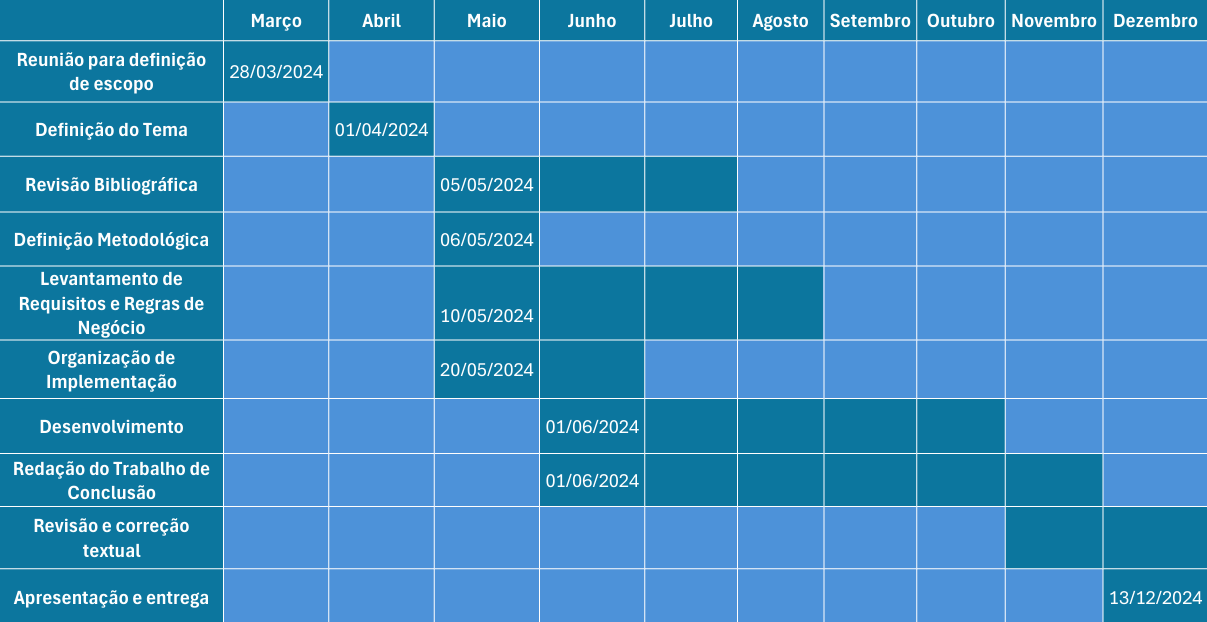
\includegraphics[width=0.8\textwidth]{imagens/cronograma1.png}
  \caption{Cronograma geral de desenvolvimento do projeto.}
  \legend{Fonte: Autor.}
  \label{fig:cronograma}
\end{figure}